describe and motivate proposed detector and beam test requirements 


\subsection{Requirements for the detector, beam and commissioning}
The Single-Phase Cern Prototype detector is intended to provide necessary information to reduce systematic uncertainties for the oscillation measurements in the US-based long base-line neutrino experiment.   The LAr TPC technology is not new but wasn't extensively used in the 1-10 GeV neutrino energy range.  The main source of uncertainties due to detector with the current values are shown in table \ref{table:deterr}


\begin{table}[h]
\centering


\caption{Current known sources of detector uncertainties for liquid argon or TPC.}
\label{table:deterr}
\begin{tabular}{|c|c|c|}

\hline
\textbf{source of uncertainty } & \textbf{value} & \textbf{reference}  \\ \hline
  e/$\gamma$ separation        &           &                   \\ \hline
  e-m shower calibration        &           &            \\ \hline
   hadronic shower calibration       &           &        \\ \hline
 .....   &   &   \\ \hline
\end{tabular}
\end{table}

With current detector uncertainties from table \ref{table:deterr} the sensitivities for the CP violation phase measurement is shown in Fig. \ref{fig:cpsensitivity}  {\bf Task: make this plot} . The  proposed test beam detector will reduce uncertainties to XX%  and improve our sensitivity to $\delta_{CP}$ as shown in Fig. \ref{fig:cpsensitivity} {\bf Task: make this plot.



\begin{figure}[h!]
  \centering
%\includegraphics[scale=0.4]{}
\label{fig:cpsensitivity}
  \caption{Sensitivites for the $\delta_{CP}$ measurement  for using current knowledge of the single-phase LAr-TPC detector technology and for reduced detector uncertainties from SPCP beamtest data.  The plots prepared for 40 kton fiducial mass and $xx\times 10^{21}$POT.}
\end{figure}

\newpage

\subsubsection{Particles energy and direction}
Plans for running beam for the the ELBNF include both neutrino and anti-neutrino configurations. These beams will be composed  mainly of muon neutrinos (anti-neutrinos) as well as electron neutrinos (anti-neutrinos). To take into account  

\begin{figure}[h!]
  \centering
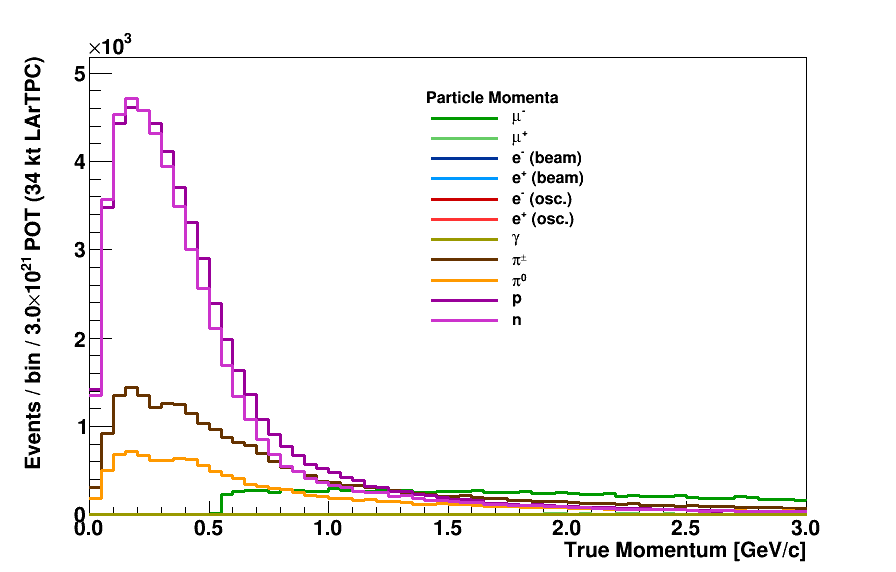
\includegraphics[scale=0.4]{figures/True_Momenta_per_Particle}
\label{fig:particle_momenta}
  \caption{Particle momenta distributions for particles coming from all fluxes ($\nu_e$, $\nu_\mu$, $\bar \nu_e$ and $\bar \nu_\mu$) at both near and far detector locations.  }
\end{figure}


\begin{figure}[h!]
  \centering
\includegraphics[scale=0.4]{figures/True_Theta_per_Particle}
\label{fig:particle_momenta}
  \caption{Particle angle wrt to the beam axis distributions for particles coming from all fluxes ($\nu_e$, $\nu_\mu$, $\bar \nu_e$ and $\bar \nu_\mu$) at both near and far detector locations.  }
\end{figure}


Plots for the  rates for the particles.
\subsubsection{Particle rates}
Estimation of the necessary for each particle type and energy bin. 
\subsubsection {Run plan}
Based of the rates from the beam and required rates from the physics considerations.




\subsection{Detector performance tests}

\subsubsection{Bethe-Bloch parametrisation of charged particles}
How we compare with Lariat. Energy scale measurement. 
Multiple scattering.  

The set of single-phase prototype detector help to understand the detector response to cosmic muons. But there is still lots to learn with additional studies. 

The charge  particle identification efficiencies  has been mapped for only limited range of the particle energies.  

\subsubsection{e/$\gamma$ separation}
\subsubsection{Reconstruction efficiencies and particle identification}



\subsubsection{Cross section measurements}
absorption, charge exchange, pions and Kaons, 
\subsubsection{Charge sign determination}

\subsubsection{Single track calibration}
\subsubsection{Shower calibration}

Charged particles pass through the 

- Hadronic shower
- Electromagnetic shower
- Missing energy (Neutrons scattering)
 

\subsection{Other measurements} 
\subsubsection{Anti-proton annihilation }
\subsubsection{Proton decay background (cosmogenic $K^{0} \to K^+$)}



